\chapter[Introdução]{Introdução}

O malte é um produto de extrema importância para diversos setores industriais, sendo o principal insumo na produção de cerveja, onde fornece açúcares fermentáveis, cor e aroma à bebida. No setor cervejeiro, o malte de cevada é o mais utilizado; no entanto, há um crescente interesse em pesquisas que buscam desenvolver malte a partir de outros grãos, como arroz, milho e trigo, visando atender demandas específicas, como a produção de cervejas livres de glúten \cite{CECCARONI2019}. Além disso, o malte tem ganhado destaque como ingrediente funcional na indústria alimentícia, sendo utilizado, por exemplo, na fabricação de pães, devido às suas propriedades nutricionais \cite{KOISTINEN2020}.

A produção de malte, no entanto, enfrenta desafios significativos, especialmente em climas quentes, onde o controle preciso de temperatura, umidade e tempo, durante as etapas de maceração, germinação e secagem, é crucial para garantir a qualidade do produto \cite{KOVALOVA2024}. O controle desses parâmetros torna a malteação um processo complexo, exigindo equipamentos especializados e sistemas automatizados para otimizar a produção. 

No contexto acadêmico e de pesquisa, a falta de equipamentos acessíveis e confiáveis para malteação em laboratório limita o desenvolvimento de estudos e inovações nesta área, evidenciando a importância de soluções de baixo custo.

Durante uma iniciação científica (IC), foi desenvolvido um protótipo inicial (\autoref{fig:malteador}), não finalizado, restando completar a montagem física e desenvolver o sistema de controle e automação. O presente trabalho dá continuidade à IC ao propor uma solução de \textit{software} responsável por garantir que o processo de malteação ocorra adequadamente. 

\begin{figure}[ht]
    \centering
    \caption{Protótipo desenvolvido durante a IC. (A) Espaço reservado para o microcontrolador; (B) Componentes eletrônicos; (C) Parafuso de revolvimento; (D) Entrada de ar; (E) Entrada de água; (F) Saída de água; (G) Sensor de dióxido de carbono, umidade e temperatura.}  
    \label{fig:malteador}
    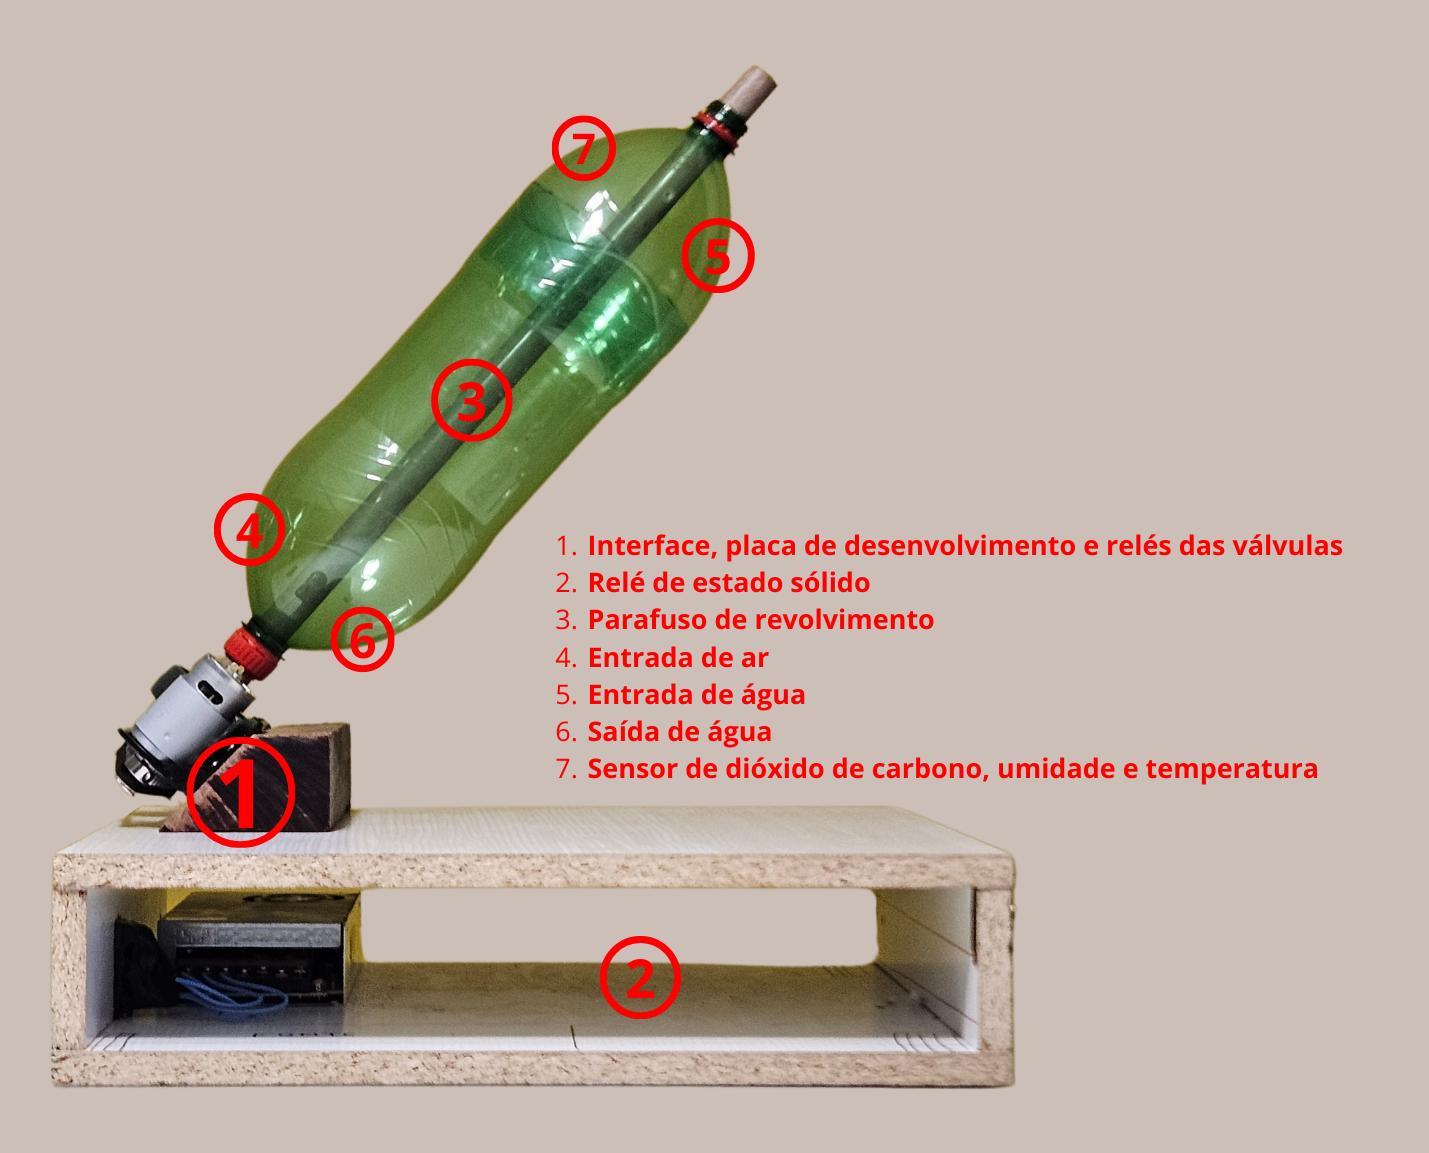
\includegraphics[width=0.8\textwidth]{Vista Lateral do Malteador.png}

    {\centering\footnotesize Fonte: Autoria própria.\par}
\end{figure}

A proposta visa o desenvolvimento de um sistema baseado no microcontrolador ESP32-C3, da fabricante chinesa Espressif Systems, integrado com um aplicativo Android (\autoref{fig:esquemamacro}). Esse microcontrolador foi escolhido por sua relação custo-benefício, capacidade de processamento e suporte a tecnologias de comunicação como Bluetooth e Wi-Fi \cite{rodrigues2021controle, santos2019sistema}. Para seu firmware, optou-se pela linguagem MicroPython, que oferece uma curva de aprendizado suave e é bastante utilizada em projetos de prototipagem rápida e Internet das Coisas (IoT) \cite{TOLLERVEY2017, brito2020automaccao}. Já o aplicativo Android foi desenvolvido em Kotlin, linguagem oficial para o desenvolvimento Android \cite{sempreupdate_kotlin_2020}.

\begin{figure}[ht]
    \centering
    \caption{Esquema geral}
    \label{fig:esquemamacro}
    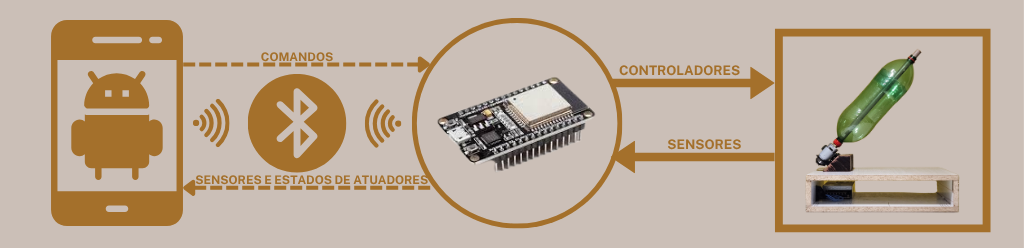
\includegraphics[width=1.0\textwidth]{esquema-macro.png}

    {\centering\footnotesize Fonte: Autoria própria.\par}
\end{figure}

Em relação à parte física do equipamento (\autoref{fig:esquemaeletronico}), o sistema conta com um motor controlado por pulsos PWM, responsável por acionar um eixo acoplado a uma hélice que realizará a movimentação dos grãos. Há também uma resistência elétrica utilizada para o aquecimento do ar, com o objetivo de atingir temperaturas entre 60$^{\circ}$C e 90$^{\circ}$C. Um compressor de ar integra o sistema para fornecer ventilação forçada, enquanto duas válvulas — uma de entrada e outra de saída — controlam o fluxo de água no equipamento. A ativação dos dispositivos é realizada por meio de relés, sendo utilizados relés de estado sólido para o motor, a resistência e o compressor, devido à sua maior robustez e compatibilidade com controle por PWM, já as válvulas são acionadas por relés mecânicos convencionais, do tipo amplamente utilizado com plataformas Arduino.

\begin{figure}[ht]
    \centering
    \caption{Esquema eletrônico do malteador}
    \label{fig:esquemaeletronico}
    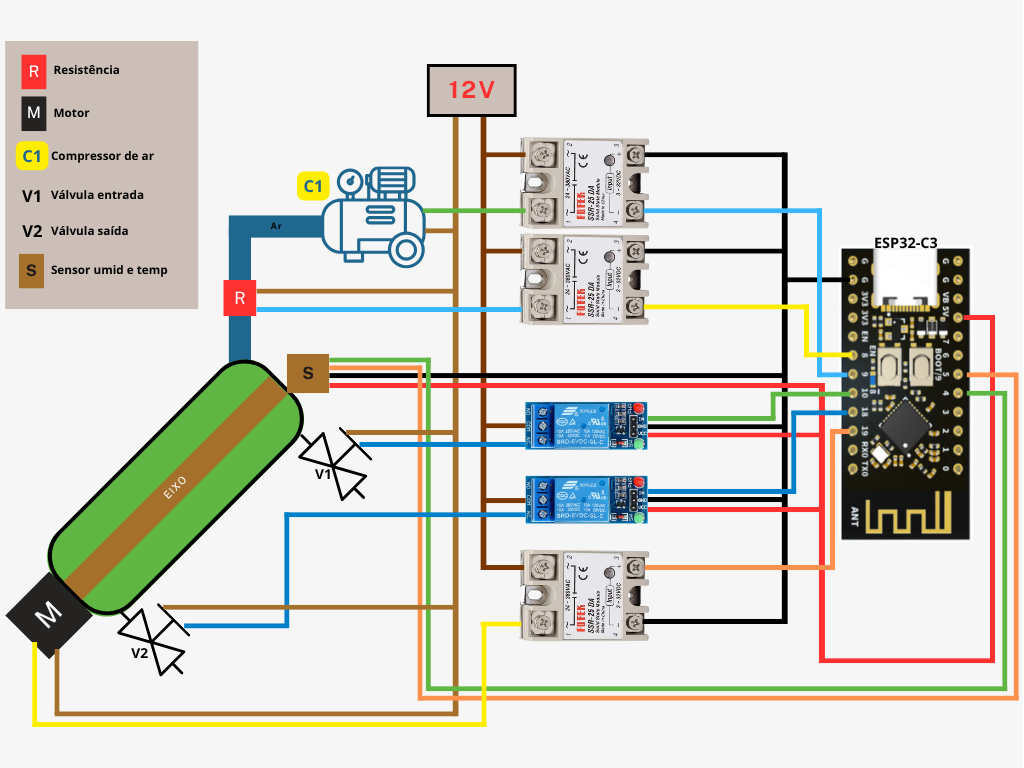
\includegraphics[width=1.0\textwidth]{esquema-eletronico-macro.png}

    {\centering\footnotesize Fonte: Autoria própria.\par}
\end{figure}

A comunicação entre o firmware e o aplicativo é realizada via Bluetooth Low Energy (BLE), uma tecnologia de baixo consumo energético e amplamente disponível em dispositivos móveis \cite{heydon2012bluetooth}, permitindo a configuração remota e o monitoramento em tempo real dos parâmetros operacionais. Além disso, a documentação dos softwares desenvolvidos pode servir como referência para outros estudos envolvendo IoT dentro do IFES, especialmente no que se refere à integração entre ESP32 e Android.

Este trabalho, também, surge a partir da demanda do Laboratório de Análise de Cervejas e Matérias-Primas (LACEMP), que busca iniciar estudos experimentais sobre o processo de malteação. Isso serviu de motivação para o desenvolvimento de um sistema que permita monitorar e controlar as variáveis do processo de forma precisa e reprodutível. 

Por fim, a automação proposta busca simplificar ao máximo a operação do equipamento e fornecer um ambiente que facilite futuras análises e ajustes nos experimentos conduzidos no LACEMP. Com isso, espera-se que esta solução de baixo custo promova avanços tanto na pesquisa acadêmica quanto no desenvolvimento de tecnologias acessíveis para a indústria cervejeira e áreas afins.